\documentclass[a4paper]{scrartcl}
\usepackage{amsmath}
\usepackage{amsfonts}
\usepackage{amssymb}
\usepackage[utf8]{inputenc}
\usepackage[frenchb]{babel}
\usepackage[T1]{fontenc}
\usepackage{lmodern}
\usepackage{graphicx}

\title{Implémentation d'un moteur physique 2D dans un langage fonctionnel}
\subtitle{Et plus encore...}

\begin{document}
\maketitle

\tableofcontents

\newpage

\section*{Introduction}
\addcontentsline{toc}{section}{Introduction}

\section{Philosophie de développement et organisation du code}
\paragraph{Un moteur purement fonctionnel}

Avec OCaml nous avons un langage fonctionnel de par son héritage et sa
conception, mais embarquant également des constructions non
fonctionnelles (références, champs mutables, …). Comme il est peu
courant de voir des jeux et ce qui s'y rapporte (moteur de jeu, moteur
physique) codés dans des langages fonctionnels (en général c'est
plutôt du C++ utilisant massivement le paradigme objet), nous avons
choisi d'implémenter le moteur de jeu, le moteur physique et les
structures sous-jacentes de manière purement fonctionnelle, et en
utilisant les idiomatismes Caml que sont les modules pour structurer
notre projet.

En pratique, comment réaliser ce qui semble intuitif avec des éléments
mutables («~on fait bouger la boule~» devient «~on modifie ses
coordonnées qui sont des champs mutables~») en n'utilisant que des
structures non mutables ?

Notre code sera en fait composé de structures (non-mutables, donc)
décrivant un monde (monde d'objets physiques par exemple). Les
fonctions agissant sur ce monde n'auront d'autre possibilité que d'en
retourner un nouveau : on aura des fonctions qui, après application
partielle, seront de type \texttt{world -> world}. Alors, il suffit
d'enchainer l'application de ces fonctions à partir d'un
\texttt{world} fraichement créé.

Pour exprimer joliment (sans trop de parenthèses partout) un tel
enchainement de «~modificateurs~», avec aussi une petite «~saveur~»
impérative, nous avons massivement utilisé l'opérateur \texttt{>>=}
défini comme suit :
\begin{verbatim}
let ( >>= ) w f = f w
\end{verbatim}

Celà semble idiot, mais ça nous permet d'enchainer très simplement des
«~effets fonctionnels~» sur une structure. Pour ajouter une balle puis
une force, on fera par exemple :
\begin{verbatim}
new_world () >>=
  add_ball x y radius >>=
  add_f gravity
\end{verbatim}

Les fonctions \texttt{add\_ball} et \texttt{add\_f} prennent un
\texttt{world} en argument et en retournent un autre, mais sa
propagation est cachée par l'opérateur.

\paragraph{Les modules pour hiérarchiser, organiser le code et
  abstraire les implémentations}

La structure du code a été dirigée par la volonté d'écrire du code le
plus généraliste possible, composé d'unités les plus indépendantes
possible les unes des autres.

Nous avons utilisé pour celà le système de modules d'OCaml. Il nous
permet ainsi , si nous avons besoin d'une unité réalisant certaines
fonctions, de définir sa signature (le type de ce qu'il y aura dedans
et les fonctions qu'elle fournit). Ensuite, on est libre d'implémenter
effectivement la signature, d'une ou plusieurs manières. On est ainsi
certain que les spécificités de l'implémentation ne se mélangeront pas
avec l'utilisation qui en est faite dans le module qui a besoin des
fonctionnalités.

Par exemple, le moteur physique utilise un module définissant un
conteneur d'objets. La signature d'un tel conteneur abstrait le type
(on n'y a pas accès de l'extérieur), et définit des opérations :
itérer sur la structure, ajouter / supprimer des éléments.

Il définit ensuite un \emph{foncteur} : un \emph{foncteur} est aux
modules ce qu'une fonction est aux valeurs OCaml : un foncteur prend
un ou plusieurs modules en argument et retourne un autre module.

Le foncteur en question, une fois qu'on lui a passé un module
définissant un conteneur, retourne un module décrivant un moteur
physique utilisant ce type de conteneur.

\begin{figure}[h]
  \centering
  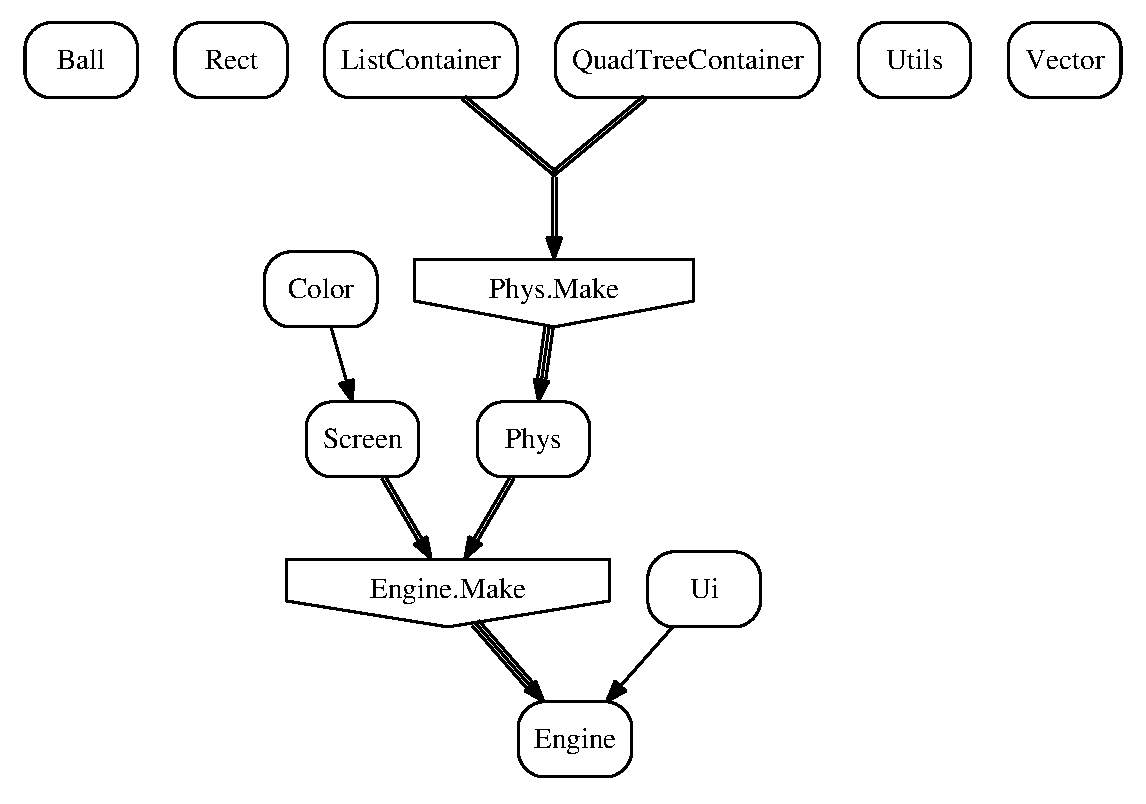
\includegraphics[scale = 0.7]{modules.eps}  
  \caption{Architecture des modules composant le projet}
  Les doubles flèches désignent l'argument d'un foncteur, les triples
  flèches la valeur de retour
  \label{fig:modules}
\end{figure}

Notre projet se structure ainsi par le bied de modules et foncteurs
OCaml. Sur la figure, certains modules ne sont pas reliés : il s'agit
de modules très généralistes qui sont en fait utilisés par à peu près
tous les autres modules (il serait illisible de les relier à tout le
monde).

\paragraph{Un moteur généraliste et réutilisable}

Notre moteur se veut par généraliste et réutilisable : il définit un
ensemble de modules, qui s'utilisent finalement comme une bibliothèque
externe.

Ainsi, il peut être exporté sans aucune modification pour une autre
utilisation, et peut être utilisé pour réaliser diverses programmes,
comme le montre la section \ref{applications}.

\section*{}
À présent, il est temps de regarder de plus près les implémentations
effectives des modules présentés. Au programme : structures de données
fonctionnelles, simulation physique et gestion des collisions.

\section{Containers de balles : les modules \texttt{ListContainer}
  et \texttt{QuadTreeContainer}}
\subsection{\texttt{ListContainer} : conteneurs utilisant des listes}

Lorsqu'il s'agit de stockée des données dans une structure de donnée permettant d'avoir toutes les données pour la restitution du monde. Il est aussi nécessaire d'avoir des fonctions associé à cette structure de donnée permettant une certaine interaction avec les éléments de ce monde, par exemple ajouter ou retirer un élément, actualiser l'élément

C'est pourquoi la première idée est de stocker  ces élément dans une liste. Cette première structure est assez simple à mettre en œuvre et ne génère pas de cas problématiques particuliers. les fonctions sont déjà définies mais dans notre cas il est nécessaire de légèrement les modifier pour avoir une structure modulaire. 
Il nous faut prendre en compte aussi la taille du monde c'est pourquoi au lieu d'avoir un type list tout simplement on a un type Vector * Vector * list.

Toutefois, bien que simple a mettre en place elle est très peu optimisée. C'est pourquoi nous allons voir une structure différente, plus complexe mais qui nous permettra d'avoir de meilleures performances.


\subsection{\texttt{QuadTreeContainer} : une structure arborescente
  pour stocker nos balles}

Les quadTree sont une structure arborescente dont les nœuds possèdent chacun 4 sous-arbre, ces sous-arbres représentent le découpage du plan en quatre parties, la partie en haut à gauche, en bas à droite, etc. Ainsi en décomposant un plan en quatre parties et en plaçant chacun de ces élément dans une de ces sous-partie nous permet d'optimiser la gestion des collisions, en effet les boules se trouvant dans un sous-arbre ne peuvent, en théorie, être en collision avec les boules d'un des trois autre sous-arbre nous limitant ainsi les calculs à effectuer.

Cependant lorsque nous avons des boules de tailles différentes, et surtout quand la différence des tailles est grande, ce principe doit être adapté car les boules de grande tailles peuvent dépasser de leur domaine.
Il s'offrait plusieurs solutions à nous, soit nous ne considérions que les centre des boules et adaptions la gestion des collision en fonction du rayon de la boule, soit nous découpions la boule en plusieurs partie pour la placer dans plusieurs feuilles et faisions en sorte d'éviter de faire un calcul pour gérer le collision entre la même boule mais situé dans plusieurs feuilles.

Trouvant ces méthodes peut satisfaisantes, par exemple pour dans le cas de la duplication des balles lors d'un dépassement de domaine peut conduire a un arbre très grand contenant beaucoup plus d'éléments que le nombre total de boules réduisant ainsi grandement la performance du quadTree, nous avons opter pour un quadTree a plusieurs niveau. C'est à dire que chaque nœud de l'arbre va contenir une liste, peut-être vide, de balles, ces balles sont celles qui ne peuvent pas être placées dans un unique sous-arbre. De ce fait les balles dont le rayon est important se trouvera peu profond dans l'arbre tandis que les balle dont le rayon est petit se trouveront généralement dans les nœuds les plus profonds de l'arbre. Par conséquent une balles pourra entrer en collision avec les balles qui sont dans le même nœud qu'elle, dans les nœuds de ses sous-arbres, et dans les nœuds de ses pères. Ceci nous permet d'avoir un bon compromis entre l'optimisation et la gestion des problématiques liées à la structure de quadTree.

Théoriquement, dans la majeur partie des cas, avec cette structure nous avons une meilleure complexité qu'avec l'utilisation des listes et dans certain cas particulier nécessitant un fort concours de circonstance une complexité équivalente avec celle des listes. Les quadTree nous permettent dans l'absolu d'avoir une complexité logarithmique au lieu d'une complexité linéaire avec les listes.

\subsection{Structures de données fonctionnelles et \emph{Zippers}}


\section{Simulation physique : module \texttt{Phys}}
[module Phys obtenu comme image du foncteur Phys.Make sur un module
conteneur]
\subsection{Monde physique, objets physique : simulation simple sans
  collisions}
\subsection{Gestion des collisions}
\paragraph{Un peu de physique}
\paragraph{En pratique}
\subsection{Ce que nous permettrait également notre monde purement
  fonctionnel}
[Gestion plus fine des collisions, backtrack / dichotomie]

\section*{}
On a maintenant un moteur physique 2D (ne gérant certes que des
balles), prenant en compte des forces, des collisions, et pouvant
s'utiliser de manière totalement indépendante. Il fournit un monde
physique (\texttt{Phys.world}) dans lequel on peut ajouter des balles,
des forces, … et dont on peut ensuite simuler l'évolution.

Ainsi, en vertu du sacro-saint principe d'isolement, ce module ne
traite pas avec l'affichage. Son rôle est simplement de simuler la
physique.

Et c'est parce que l'on veut quand même pouvoir afficher des choses à
l'écran qu'intervient...

\section{Le module \texttt{Engine} : un moteur de jeu}

[ce qu'on appelle moteur de jeu est en réalité un module gérant tout
ce qui touche à la physique, l'affichage, et qui permet à
l'utilisateur de programmer aisément des situations variées]

Le module Engine est le module avec lequel traitera au final
l'utilisateur : il doit principalement permettre de simuler la
physique et fournir une sortie graphique quelconque. Son rôle est en
fait d'agencer les deux mondes : «~brancher~» le moteur physique, qui
ne connaît rien de l'affichage, sur un module dédié à l'affichage, qui
lui ne connaît rien des objets physiques.

La pièce centrale d'\texttt{Engine} est donc une fois encore un
foncteur, \texttt{Make}, prenant en argument un module contenant un
moteur physique (\texttt{Phys}, par exemple) et un autre module
fournissant une sortie graphique.

Nous avons ici implémenté un module \texttt{Screen} ayant ce rôle,
mais il est tout à fait possible (hypothétiquement) d'écrire un module
réalisant par exemple la sortie graphique dans une vidéo

\subsection{Module \texttt{Screen} : affichage à l'écran}
Le module \texttt{Screen} est une implémentation satisfaisant la
signature qu'\texttt{Engine.Make} attend pour un module
d'affichage. Il permet ainsi d'abstraire l'utilisation du module
\texttt{Graphics}, lui même place d'un joyeux bazar puisqu'il condense
plein de fonctionnalités a priori sans rapport.

Le contenu de \texttt{Screen} est en pratique peu intéressant,
puisqu'il ne s'agit que d'une surcouche aux fonctions de dessin de
\texttt{Graphics}. Il définit un buffer d'affichage, contenant la
taille de l'écran et des informations spécifiques à l'implémentations
(cachées dans un type abstrait par la signature), comme le
\emph{double buffering} (activé).

Connaître la taille du buffer d'affichage est notamment important pour
les modules «~au dessus~», utilisant ce module ci : par exemple, le
module \texttt{Engine} en fait usage pour synchroniser (si l'option
\texttt{borders\_follow\_buffer\_size} est à \texttt{true}) les bordures
physiques avec la taille de l'écran, ce qui permet de pousser les
boules en modifiant la taille de la fenêtre \footnote{On peut
  notamment faire ceci dans les exemples du programme \texttt{main}}

\subsection{Que fait exactement \texttt{Engine} ?}
\texttt{Engine} fait la liaison entre la simulation et l'affichage :
il fournit tout d'abord son propre monde (\texttt{Engine.world}),
servant de surcouche au module gérant la physique.

Par ailleurs, il fournit 
\begin{itemize}
\item Une fonction \texttt{draw} permettant de dessiner les objets
  physiques sur l'écran
\item Une fonction \texttt{run} permettant de «~faire tourner~» le
  programme, une fois que l'on a ajouté ce qu'il faut au monde, en
  affichant au nombre d'images par seconde désiré son évolution
\end{itemize}

\subsection{Le système de \emph{hooks}}
Avec seulement ceci, la personnalisation serait un peu pauvre : on
pourrait ajouter diverses balles, des forces, mais ensuite il ne
serait possible que de regarder leur évolution sans pouvoir
intervenir.

Pour pouvoir intervenir aisément, et simuler tout type de
comportements, nous avons mis en place un système de \emph{hooks} : le
module \texttt{Engine} permet à l'utilisateur de donner au module des
fonctions que le module exécutera à un moment précis.

Par exemple, \texttt{Engine} fournit des \texttt{predraw\_hooks} :
l'utilisateur indique un ensemble de fonctions d'affichage qu'il veut
voir exécutées avant le dessin des boules, lui permettant d'afficher
par exemple un fond personnalisé \footnote{Ceci est utilisé notamment
  dans les programmes \texttt{billard} et \texttt{missileCommand}}.
Existent également les hooks :
\begin{itemize}
\item \texttt{postdraw\_hooks} : fonctions d'affichage à exécuter à la fin
\item \texttt{ball\_hook} : permet de définir une fonction
  personnalisée pour afficher les balles \footnote{Utilisé dans
    \texttt{billard} pour ajouter un cercle autour des boules, et bien
    entendu dans \texttt{missileCommand} pour dessiner les astéroïdes}
\item \texttt{user\_action} : un hook très important : il est appelé
  dans la boucle principale (tous les \emph{dt} donc) et permet de
  modifier le monde à volonté
\end{itemize}

\subsection{Historique des collisions}
Toujours dans l'objectif de pouvoir utiliser le moteur à notre guise,
est fourni un historique des collisions via une file (utilisant le
module \texttt{Queue} de la bibliothèque standard OCaml). Ceci permet
à l'utilisateur du moteur de réagir éventuellement en cas de
collision, s'il veut agir sur les balles en question. C'est par
exemple utilisé dans \texttt{missileCommand} pour éliminer les
astéroïdes touchant le sol, et pour compter les points lorsque l'on
touche un astéroïde.

\subsection{Gestion de l'entrée utilisateur}
Nous avons également besoin de gérer les entrées utilisateur : on veut
pouvoir réagir quand l'utilisateur appuie sur une touche, clique sur
un bouton de la souris ou encore effectue un \emph{slide} (un
cliqué-glissé).

C'est à nouveau le module \texttt{Graphics} qui nous permet
d'implémenter ceci, mais comme à notre habitude on va abstraire ceci
dans un module : \texttt{Ui}.

Celui-ci va nous fournir, lors de l'appel à la fonction
\texttt{get\_status}, une liste des évènements apparus depuis le
dernier appel : appui sur un bouton, cliqué-glissé, etc.

C'est le module \texttt{Engine} qui va ensuite utiliser ce module, et
passera au \emph{hook} \texttt{user\_action} la liste des évènements
apparus.

\subsection*{}
Nous avons ainsi un joli moteur de jeu tout beau, tout propre. Pour
programmer un scénario quelconque, il suffit de créer un nouveau
monde, d'ajouter nos balles, nos forces, de définir nos fonctions de
dessin et nos \emph{hooks} éventuels, puis de lancer la simulation.


\section{Application : on utilise notre moteur}
\label{applications}

\subsection{Quelques situations d'exemple}

Nous avons programmé tout d'abord quelques situations assez simples,
visant en premier lieu à tester les capacités de simulation physique
du moteur. Celles-ci sont regroupées dans le programme \texttt{main},
et peuvent être choisies dans le menu.

Elles ne font pas usage des \emph{hooks} ou autres joyeusetés, et se
contentent d'ajouter des boules, de régler le coefficient de
restitution des chocs et de mettre différentes forces.

On remarque (grâce à l'afficheur d'images par seconde dotamment - en
haut à droite) que si l'on modifie le programme \texttt{main} pour
utiliser le conteneur utilisant des listes à la place des quadTrees,
la situation «~stress test~» est beaucoup plus lente - le quadTree
optimise en effet les calculs de collisions pour un nombre important
de balles.

\subsection{Le billard}

Cette fois-ci, il s'agit d'un programme utilisant des fonctionnalités
un peu plus avancées du moteur : un \texttt{predraw\_hook} est mis
pour afficher le fond, et on utilise dans le hook
\texttt{user\_action} les évènements \texttt{Sliding} provenant du
module \texttt{Ui} pour permettre de propulser la balle blanche en
cliquant-glissant.

On notera également l'ajout de forces un peu plus fines que sur les
autres exemples : pour tenter d'avoir un rendu le plus réaliste
possible, nous ajoutons une force de frottement fluide, ainsi qu'une
force de frottement solide.

\subsection{MissileCommand : protégez votre base spatiale !}

Il s'agit du dernier programme utilisant notre moteur, et utilisant
ses fonctionnalités les plus poussées !

MissileCommand est inspiré du jeu d'arcade éponyme, édité par Atari en
1980, où l'on doit protéger notre base de missiles arrivant de
l'espace. Ici, dans ce nouvel opus remis au goût du jour\footnote{le
  21 Décembre 2012 plus précisément} il ne s'agit plus de missiles
mais de météorites, et bien entendu on joue sur la physique et les
collisions pour les repousser.

Ainsi, en cliquant on lance un projectile qui repousse les météorites
afin qu'ils ne tombent pas sur notre base. Tirer des projectiles fait
perdre de l'argent (et des points), tandis qu'on en gagne en
repoussant des astéroïdes. L'objectif est bien entendu de protéger la
base.

On utilise ici toutes les fonctionnalités de notre moteur :
\texttt{predraw\_hooks} pour afficher le fond, lecture du journal de
collisions, et modification de la fonction d'affichage des balles pour
dessiner les astéroïdes.

\end{document}
